\chapter{Revisão Bibliográfica e Estado da Arte}
\label{cap:refbib}

Neste trabalho, o objetivo foi desenvolver um multímetro capaz de medir tensão e corrente simultaneamente e enviar os dados para um smartphone por meio de uma conexão wifi. Considerando essa proposta, foram analisadas duas opções para servir como base: um multimedidor e um multímetro.

O multimedidor é um dispositivo geralmente trifásico, que permite a medição simultânea de tensão e corrente, exibindo as formas de onda em um display. Possui três ou mais canais simultâneos. No entanto, apresenta a limitação de possuir apenas um referencial de medição, com resolução na ordem de 1V nos modelos mais baratos e 0,1V nos modelos mais caros, repetindo-se esses valores para a resolução da corrente \cite{fluke434}.

Por outro lado, o multímetro é um dispositivo monofásico que permite a medição de apenas um canal por vez, como tensão, corrente, resistência, capacitância, entre outros. Ele não exibe as curvas na tela, fornecendo apenas os valores. A resolução varia, sendo que nos modelos mais simples pode chegar a 0,1 mV, enquanto a resolução da corrente é da ordem de 1uA \cite{et1100}.

Considerando que o dispositivo deve ser utilizado como uma ferramenta didática em sala de aula, é essencial que a resolução seja adequada para o bom aproveitamento das disciplinas. Além disso, a apresentação das formas de onda também é relevante. Assim, optou-se por uma abordagem que combina características de ambos os dispositivos, utilizando os diagramas de blocos para identificar as funcionalidades e suas relações com o dispositivo a ser produzido.

Para o multimedidor, foi utilizado o diagrama de blocos do \textit{oZm3} (\autoref{fig:ozm3flowchart}), um produto \textit{open source} (projeto aberto) já introduzido no mercado, sendo uma versão trifásica de outro, também \textit{open source} chamado \textit{(openZmeter)}. Ambos possuem interface de apresentação dos dados via uma página do navegador de um celular ou computador.

\begin{figure}[h]
    \caption{Diagrama de blocos do multimedidor trifásico oZm3}
    \label{fig:ozm3flowchart}
    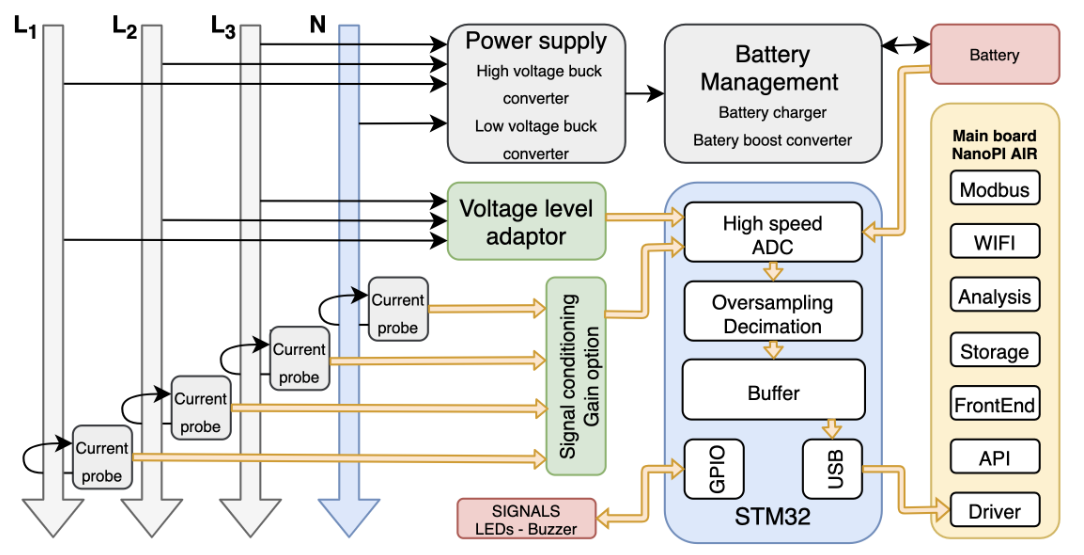
\includegraphics[width=0.8\textwidth]{figuras/openzmeter-diagrama.png}
    \fonte{\cite{3ph-ozm}}
\end{figure}

Para o multímetro, foi utilizado um diagrama de blocos (\autoref{fig:multimeterflowchart}) disponível no site da \textit{Texas Instruments}, que explica o funcionamento de um produto completo.

\begin{figure}[h]%% Ambiente figure
    %\captionsetup{width=0.55\textwidth}%% Largura da legenda
    \caption{Exemplo de um Diagrama de Blocos de um Multímetro de Bancada}%% Legenda
    \label{fig:multimeterflowchart}%% Rótulo
    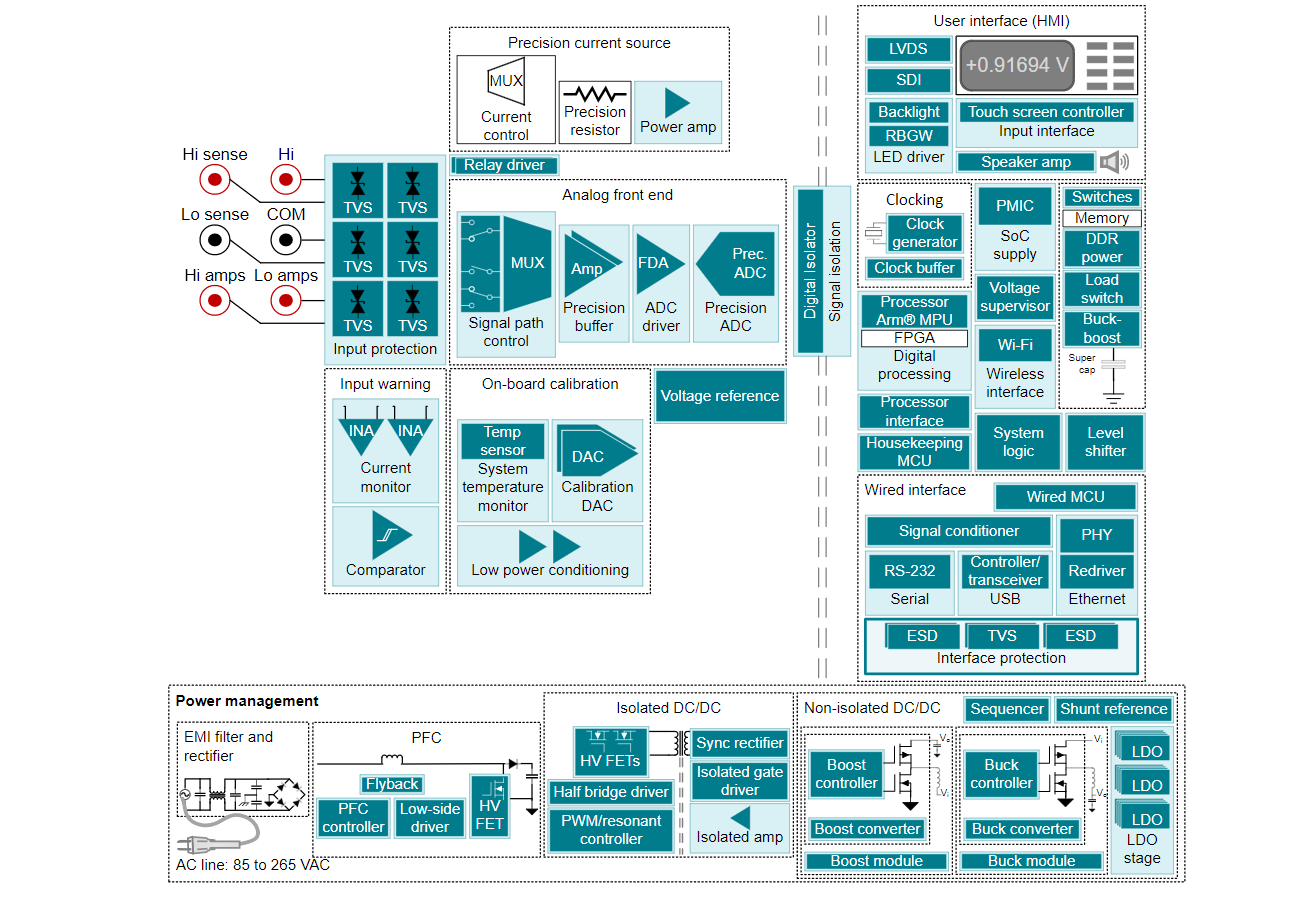
\includegraphics[width=1\textwidth]{flowchart}%% Dimensões e localização
    \fonte{\cite{DMMTI}}%% Fonte
\end{figure}

Sobre o estado da arte, existem diversos dispositivos que atendem a necessidades diferentes, como por exemplo, segurança (CAT rating), resolução, precisão ou até mesmo confiabilidade de leitura em condições de temperaturas elevadas, entre vários outros. Adicionalmente, existem também inúmeros fornecedores, tanto regionais, nacionais como internacionais, salientando a diversidade de produtos.

Dispositivos como o Fluke 28-II EX possuem boa métrica de confiabilidade e também são portáteis, além de fazerem medidas em \textit{True-RMS} (True Root Mean Square). Este dispositivo é muito benquisto, tendo boas avaliações no mundo inteiro.

\begin{figure}[htb]%% Ambiente figure
    %\captionsetup{width=0.55\textwidth}%% Largura da legenda
    \caption{Fluke 28-II}%% Legenda
    \label{fig:Fluke28-II}%% Rótulo
    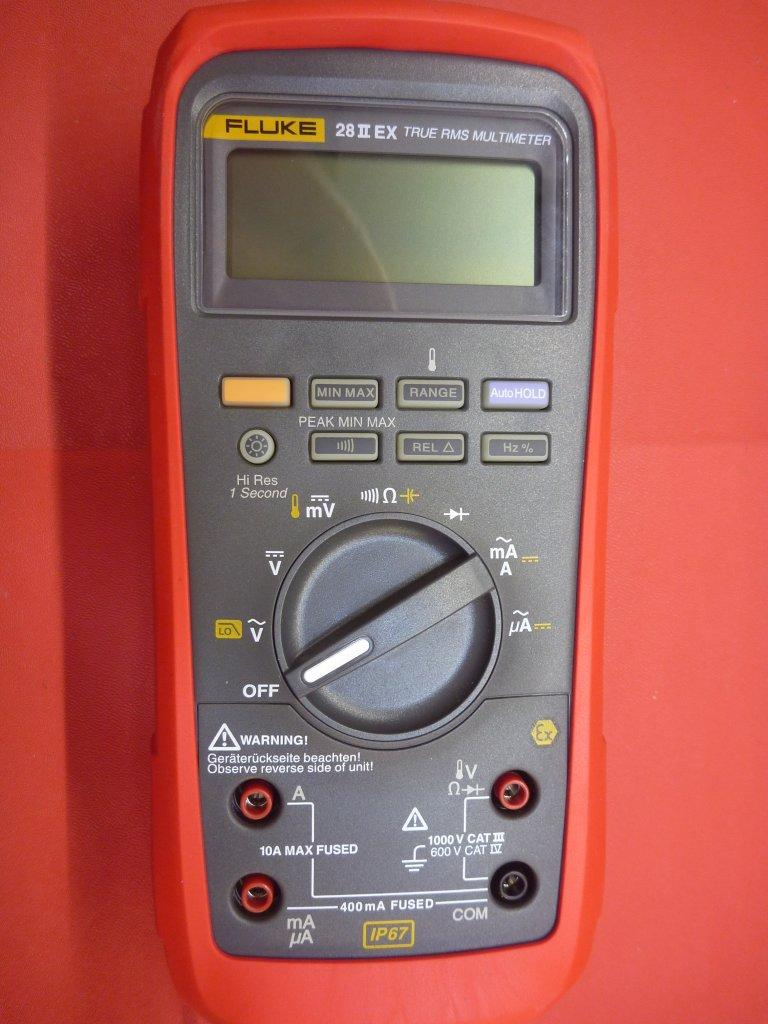
\includegraphics[scale=0.4]{Fluke28-II}%% Dimensões e localização
    \fonte{fluke28iixd}%% Fonte
\end{figure}

Sobre multímetros digitais, também existem aqueles que são de bancada ou \textit{benchtop}. Tais dispositivos são de uso mais específico, prezando a precisão de leitura, resolução e também contendo algumas \textit{features} a mais. Como exemplo, o DMM7510 7.5 Digit Graphical Sampling Multimeter da Tektronix é um dispositivo que porta todas as funções já explicitas e também várias outras de uso extremamente específico, como \textit{profiling} de corrente de consumo de energia em dispositivos \gls{IoT} (\textit{Internet of Things}), como mostrado na \autoref{fig:tektronixdmm}.

\begin{figure}[htb]%% Ambiente figure
    %\captionsetup{width=0.55\textwidth}%% Largura da legenda
    \caption{Gráfico de corrente de consumo de um dispositivo, feito pelo DMM7510 7.5 Digit Graphical Sampling Multimeter}%% Legenda
    \label{fig:tektronixdmm}%% Rótulo
    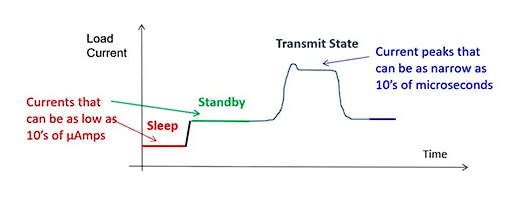
\includegraphics[scale=0.8]{tektronixdmm}%% Dimensões e localização
    \fonte{tektDMM}%% Fonte
\end{figure}

No caso de multimedidores, que são somente de uso específico industrial, alguns fornecedores e dispositivos se sobressaem, como a WEG. O MMW03, por exemplo, é um multimedidor da família MMW, fornecido pela mesma, que faz todas as medidas de grandezas elétricas no meio industrial, tem a função de parametrizá-las por meio de aplicativos \gls{IoT}, identifica sequência e falta de fases, entre outras várias funções que são benéficas para tal aplicação. 

\begin{figure}[htb]%% Ambiente figure
    %\captionsetup{width=0.55\textwidth}%% Largura da legenda
    \caption{Dispositivo MMW03}%% Legenda
    \label{fig:mmw03weg}%% Rótulo
    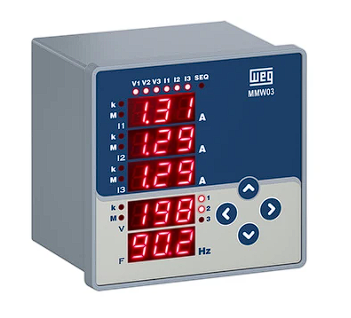
\includegraphics[scale=0.6]{mmw03weg}%% Dimensões e localização
    \fonte{WEG}%% Fonte
\end{figure}
%https://www.fluke.com/en/product/intrinsically-safe/fluke-28-ii-ex (Fluke 28-II EX)
%https://www.tek.com/en/products/keithley/digital-multimeter/dmm7510 (Benchtop DMM)
%https://www.testmart.com/webdata/mfr_pdfs/FLU/27______smeng0100.pdf (Handheld, old DMM)
%https://www.weg.net/catalog/weg/BR/pt/Automa%C3%A7%C3%A3o-e-Controle-Industrial/Controls/Prote%C3%A7%C3%A3o-de-Circuitos-El%C3%A9tricos/Multimedidores-e-Medidores-Inteligentes/Multimedidor-de-Grandezas-El%C3%A9tricas-MMW03/MULTIMEDIDOR-MMW03/p/14386964 (Multimedidor)